\documentclass[../Cours.tex]{subfiles}
\usepackage{multicol}
\usepackage[thicklines]{cancel}

\begin{document}

\setcounter{chapitre}{32}
\chapitre{Probabilités et statistiques}

\partie{Probabilités : modélisation de l'aléatoire}

\definition{Une expérience est dite aléatoire lorsqu'il est impossible de prévoir à l'avance le résultat de l'expérience.}

\exemple{Pile ou face : on ne peut savoir à l'avance sur quoi la pièce va tomber}

\definition{Une issue est un des résultats possibles de l'expérience aléatoire.}

\exemple{Dans le cas d'un lancer de dé à 6 faces, les issues sont : 1;2;3;4;5;6}

\definition{La probabilité d'une issue est un nombre entre 0 et 1.}

\exemple{Dans le cas d'un lancer de dé à 6 faces, $p\left(avoir~un~4\right) = \dfrac{1}{6}$ se lit << la probabilité d'avoir un 4 est de 1 chance sur 6 >>.}

\clearpage

\begin{questions}
\exercice\\ Dans un jeu de cartes de 32 cartes classiques, Victor choisit au hasard une carte dans le paquet.
\question Quel est le nombre d'issues possibles ?
\question Quelle est la probabilité de tirer un valet de carreau ?
\question Quelle est la probabilité de tirer une carte trèfle ?

\exercice\\ Une urne opaque contient trois boules rouges et deux boules bleues, indiscernables au toucher. Laure tire au hasard une boule dans l'urne.
\question Quelle est la probabilité de tirer une boule rouge ?
\question Quelle est la probabilité de tirer une boule bleue ?
\question Donner les deux résultats précédents sous forme de pourcentage.

\exercice\\ Une roue est divisée en trois secteurs de couleurs différentes. Jérôme fait tourner la roue.

\def\centerarc[#1](#2)(#3:#4:#5)% Syntax: [draw options] (center) (initial angle:final angle:radius)
    { \draw[#1] ($(#2)+({#5*cos(#3)},{#5*sin(#3)})$) arc (#3:#4:#5); }


\question Pourquoi peut-on dire les trois couleurs ont autant de chances d'être obtenues ?
\question Quelle est la probabilité d'obtenir une des trois couleurs ? Donner le résultat sous forme de fraction, de nombre décimal et de pourcentage.

\begin{center}
    \begin{tikzpicture}[0.8]
        \draw (0,0) circle (1);
        \draw[rouge,fill=rouge] (1,0) -- (0,0) -- ({cos(120)},{sin(120)});
        \draw[vert,fill=vert] ({cos(120)},{sin(120)}) -- (0,0) -- ({cos(240)},{sin(240)});
        \draw[bleu,fill=bleu] ({cos(240)},{sin(240)}) -- (0,0) -- ({cos(360)},{sin(360)});
        \centerarc[fill=rouge](0,0)(0:120:1)
        \centerarc[fill=vert](0,0)(120:240:1)
        \centerarc[fill=bleu](0,0)(240:360:1)
        \draw[fill=noir] (0,1) -- (0.1,1.2) -- (-0.1,1.2) -- cycle;
    \end{tikzpicture}
\end{center}

\exercice \\ Sur les 6 faces d'un dé standard, on inscrit les lettres du mot TOUPIE.
\question Quelles sont les issues de l'expérience ?
\question Donner la probabilité de chacune des lettres possibles sous forme de fraction.

\begin{figure}[h!]
    \centering
    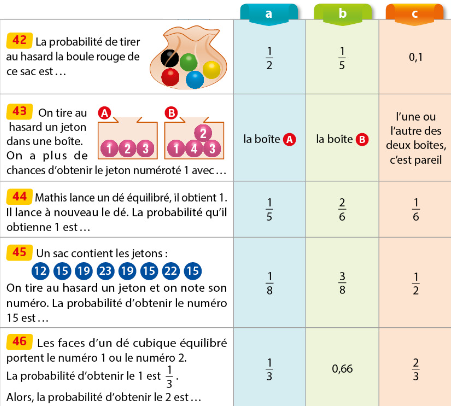
\includegraphics[scale=1]{5 - Cinquieme/chapitres/qcm_2406.png}
\end{figure}

\end{questions}


\end{document}